\documentclass[12pt, oneside]{article}   	% use "amsart" instead of "article" for AMSLaTeX format

%%%%%%%%%%%%%%%%%%%%%%%%%%%%%%%%%%%%%%%%%%%%%%%%%%%%
% set up packages, geometry
%%%%%%%%%%%%%%%%%%%%%%%%%%%%%%%%%%%%%%%%%%%%%%%%%%%%
\usepackage{geometry, textcomp, amsmath, graphicx, amssymb,fancyhdr,subcaption,bm}                
	
\geometry{letterpaper, marginparwidth=60pt}                   		
\usepackage[superscript,noadjust]{cite} % puts dash in citations to abbreviate
%\usepackage [autostyle, english = american]{csquotes} % sets US-style quotes
%\MakeOuterQuote{"} % sets quote style

\usepackage{hyperref}
\hypersetup{
    colorlinks=true,
    linkcolor=blue,
    filecolor=magenta,      
    urlcolor=cyan,
}

\usepackage{etoolbox}
\AtBeginEnvironment{quote}{\small}

\usepackage{float,color}

\usepackage{pgf, tikz, eqnarray}
\usetikzlibrary{arrows, automata}
%%%%%%%%%%%%%%%%%%%%%%%%%%%%%%%%%%%%%%%%%%%%%%%%%%%%

%%%%%%%%%%%%%%%%%%%%%%%%%%%%%%%%%%%%%%%%%%%%%%%%%%%%
\pagestyle{plain}                                                      %%
%%%%%%%%%% EXAFT 1in MARGINS %%%%%%%                                   %%
\setlength{\textwidth}{6.5in}     %%                                   %%
\setlength{\oddsidemargin}{0in}   %% (It is recommended that you       %%
\setlength{\evensidemargin}{0in}  %%  not change these parameters,     %%
\setlength{\textheight}{8.5in}    %%  at the risk of having your       %%
\setlength{\topmargin}{0in}       %%  proposal dismissed on the basis  %%
\setlength{\headheight}{0in}      %%  of incorrect formatting!!!)      %%
\setlength{\headsep}{0in}         %%                                   %%
\setlength{\footskip}{.5in}       %%                                   %%
%%%%%%%%%%%%%%%%%%%%%%%%%%%%%%%%%%%%                                   %%		

%%%%%%%%%%%%%
% DEFINE CODE BLOCK
%%%%%%%%%%%%%
\usepackage{listings}

\definecolor{dkgreen}{rgb}{0,0.6,0}
\definecolor{gray}{rgb}{0.5,0.5,0.5}
\definecolor{mauve}{rgb}{0.58,0,0.82}

\lstset{frame=tb,
  language=R,
  aboveskip=3mm,
  belowskip=3mm,
  showstringspaces=false,
  columns=flexible,
  basicstyle={\small\ttfamily},
  numbers=none,
  numberstyle=\tiny\color{gray},
 % keywordstyle=\color{blue},
  commentstyle=\color{dkgreen},
  stringstyle=\color{mauve},
  breaklines=true,
  breakatwhitespace=true,
  tabsize=3,
  otherkeywords={0,1,2,3,4,5,6,7,8,9},
  deletekeywords={data,frame,length,as,character,dunif,ps},
}

\begin{document} 

\section*{Numerical Approach to Optimal Control Problem in King and Roughgarden 1982}

For a control problem 
\begin{align}
\max_{u} &  \int_{t_0}^{t_1} f(t,x(t),u(t)) dt \nonumber \\
\mathrm{subject\ to\ } & x'(t) = g(t,x(t),u(t), \nonumber \\ 
& x(t_0) = x_0\ \mathrm{and}\ x(t_1)\ \mathrm{free}
\end{align}

we construct the Hamiltonian $H$, and use this to generate the necessary conditions for the optimal control problem. The Hamiltonian is defined as
\begin{align}
H(t,x,u,\lambda) = f(t,x,u) + \lambda g(t,x,u).
\end{align}

The necessary conditions in terms of the Hamiltonian are the (1) optimality condition, (2) adjoint equation, and (3) transversality condition.

\begin{align}
&\frac{\partial H}{\partial u} = 0\ \mathrm{at}\ u^* \\
&\lambda'(t) = -\frac{\partial H}{\partial x} \\
&\lambda(t_1) = 0
\end{align}

The optimal control problem we are interested in is
\begin{align}
\max_{u} &  \int_0^T \frac{1}{T} \log( x_2(t) ) dt \nonumber \\
\mathrm{subject\ to\ } & \dot{x_1} = u(t) x_1,\ \dot{x_2} = (1-u(t)) x_1, \nonumber \\ 
& x_1(0) > 0,\ x_2(0) \geq 0,\\
& 0 \leq u(t) \leq 1.
\end{align}

This is equivalent to solving the problem with the following objective function:
\begin{align}
\max_{u} &  \int_0^T  \log( x_2(t) ) dt 
\end{align}

The Hamiltonian here is:
\begin{align}
H = \log( x_2(t) ) + x_1( \lambda_1 - \lambda_2 ) u(t) + x_1 \lambda_2
\end{align}

If season length is uniformly distributed over, season length factors out of the objective function. The objective function is independent of the control . For this problem, the optimality condition is 
\begin{align}
\frac{\partial H}{\partial u} = x_1(\lambda_1 - \lambda_2) = 0\ \mathrm{at}\ u^*.
\end{align}

The transversality condition is
\begin{align}
\lambda_1(T) = \lambda_2(T) = 0.
\end{align}

The adjoint equations are

\begin{align}
&-\frac{\partial H}{\partial x_1} = \dot{\lambda_1}  = u(\lambda_2 - \lambda_1) - \lambda_2 \nonumber \\
&-\frac{\partial H}{\partial x_2} = \dot{\lambda_2}  = -\frac{ 1 } {x_2}.
\end{align}


We use a forward-backward sweep algorithm (Lenhart and Workman (p. 50)) to solve this problem: 

\begin{enumerate}
\item Make a guess for the control $\vec{u}$ over the interval $[0,T]$.
\item Use the initial conditions $x_1(0) = a > 0$ and $x_2(0) = b \geq 0$ and the values for the initial guess $\vec{u}$ to solve for $\vec{x_1}$ and $\vec{x_2}$ forward in time using the differential equations in the optimality system. We solve the system of ordinary differential equations given by $g(t,x(t),u(t))$ with the initial conditions for the state variables and the initial guess for the control. The solution gives the dynamics of the state variables through time when the control is the initial guess $\vec{u}$.
\item Use the transversality condition and solve lambda backward in time according to the differential equations in system of adjoint equations. The transversality condition $\lambda(T) = 0$ provides initial values for the differential equations, which solve $\lambda'(t)$ from $T$ to $0$ using the values $\vec{x}$ and $\vec{u}$. The solution gives the dynamics of the adjoint variables through time.
\item We then use the Maximum Principle solution to update the control $u(t)$. To accomplish this, solve the optimality condition $\frac{\partial H}{\partial u} = 0$ for $u$. Use the solutions for $\vec{x}$ (Step 2) and $\vec{\lambda}$ (Step 3) to obtain new values for $\vec{u}$. In order to facilitate convergence, we update $\vec{u}$ proportional to the gradient of the Hamiltonian. Rather than updating by a convex combination of the old and new controls (as in Lenhart and Workman), here we move towards the new optimal control in proportion to the gradient of the Hamiltonian (the switch function).
\item Finally, we check for convergence. If the values for the control for the previous and current iteration are similar, we accept the values for the control as the optimal control. If the values for the control for the previous and current iteration are not similar, we return to Step 2.
\end{enumerate}

\section*{Solving the Problem with a Modified Forward-Backward Sweep in R}

\noindent The system of differential equations $\dot{\bm{x}}$ for $0\leq t \leq T$ is written as a function that computes the values of derivatives in the ODE system at time $t$:

\begin{lstlisting}
## Function that computes values of derivatives in the ODE system for state variables
## Takes the time step, system of differential equations, parameters
## The control u(t) must be an externally defined function [uFunc(t)]
derivs=numeric(2); 
forward <- function(times0,y,parms,f1,...) {

# x1 and x2 are the two entries in y (ode)
x1=y[1]; 

# control function calculated f1 at different time points
u <- f1(times0);

derivs = c(u*x1,(1-u)*x1) 
return(list(derivs));
}
\end{lstlisting}

\noindent The system of differential equations $\dot{\bm{\lambda}}$ for $0\leq t \leq T$ is written as a function that computes the values of derivatives in the ODE system at time $t$:

\begin{lstlisting}
## Function that computes values of derivatives in the ODE system for adjoint variables
## Takes the time step, system of differential equations, parameters
## The state x(t) must be an externally defined function [xFunc(t)]
backward = function(t,y,parms,f1,f2) {

lambda1=y[1];
lambda2=y[2];
u = f1(t);
x2 = f2(t);

return(list(c((lambda2-lambda1)*u - lambda2, -(1/x2) )))
}
\end{lstlisting}

\noindent We make an initial guess for the control $u(t)$ over the time interval. 

\begin{lstlisting}
# Number of time steps
# t is also used in control() and optim_fun()
nt = 101;

# initial guess for control u over the interval
uVals_init = runif(nt);
\end{lstlisting}

\noindent We fit a spline to the initial guess, which gets used in solving the ODEs for the state variables forward in time.

\begin{lstlisting}
# Using current u(t) solve forward for new x(t)
uFunc=splinefun(tVals,uVals); 
out = ode(xA,tVals,forward,parms=parmsA, atol = 1e-7, f1 = uFunc); 
new_xVals = out[,c(2,3)] 
\end{lstlisting}

\noindent We fit a function (interpolation) to the state variable for reproductive biomass ($x_2$). We used this function and the function for the control $u$ to solve the ODEs for the adjoint variables backward in time.

\begin{lstlisting}
# Using current u(t) and x(t), solve backwards for new lambda(t) 
xFunc = approxfun(tVals,new_xVals[,2]);	
out = ode(c(0,0),rev(tVals),backward,parms=parmsA , f1 = uFunc, f2 = xFunc)
new_lambdaVals = list(rev(out[,2]),rev(out[,3]) )
\end{lstlisting}

\noindent We update the control $u(t)$ using the Maximum Principle solution ($\frac{\partial H}{\partial u} = 0$) and move towards the new optimal control in proportion to the gradient of the Hamiltonian (the switch function).
. We also bound values of the control on $[0,1]$

\begin{lstlisting}
# update control u(t), using Maximum Principle solution 
switch = new_xVals[,1]*(new_lambdaVals[[1]]-new_lambdaVals[[2]])

# calculate new control with old control and gradient of Hamiltonian
new_uVals = uVals + 0.01*switch
new_uVals[new_uVals<0]=0
new_uVals[new_uVals>1]=1
\end{lstlisting}

\noindent Finally, we check for convergence and either exit the loop, or update the control and continue the loop:

\begin{lstlisting}
delta = abs(uVals - new_uVals)
stop_criteria = max(delta)
uVals = new_uVals
\end{lstlisting}

\begin{figure}[h]
   \centering
       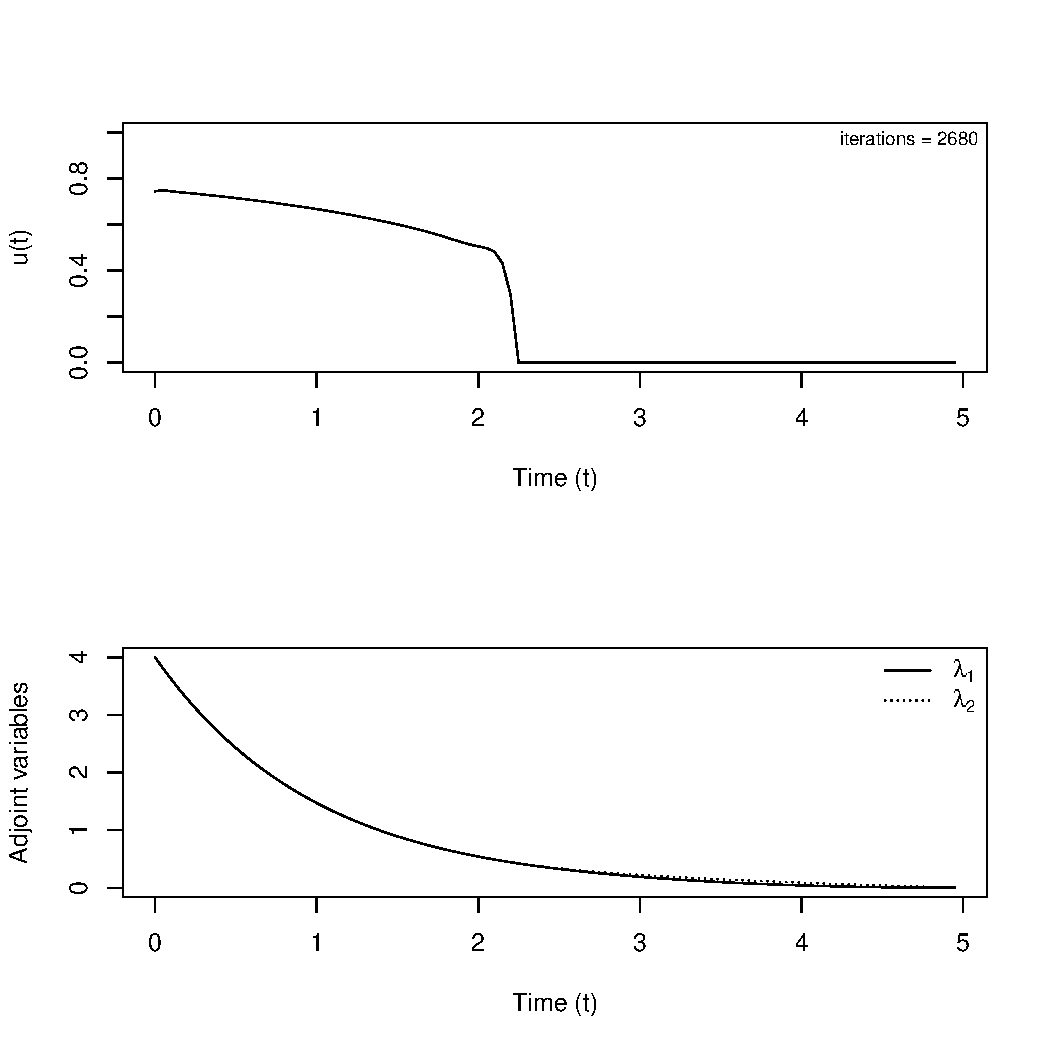
\includegraphics[page=1,width=.9\textwidth]{../../figures/forwardBackwardSweep-x1=1-x2=025}  
    \caption{ (A) The left panel shows the control $u(t)$ that maximizes $\int_{0}^{T} log(x_2) dt.$ Here, $T=5$ and $x_2(0)/x_1(0) = 0.25$. (B) The right panel shows the solution to the ODE for the control $u(t)$. [This figure corresponds to Figure 1 in King and Roughgarden (1982).] }
 \label{fig:kingRoughgardenFigure1}
\end{figure}

 \begin{figure}[h]
   \centering
       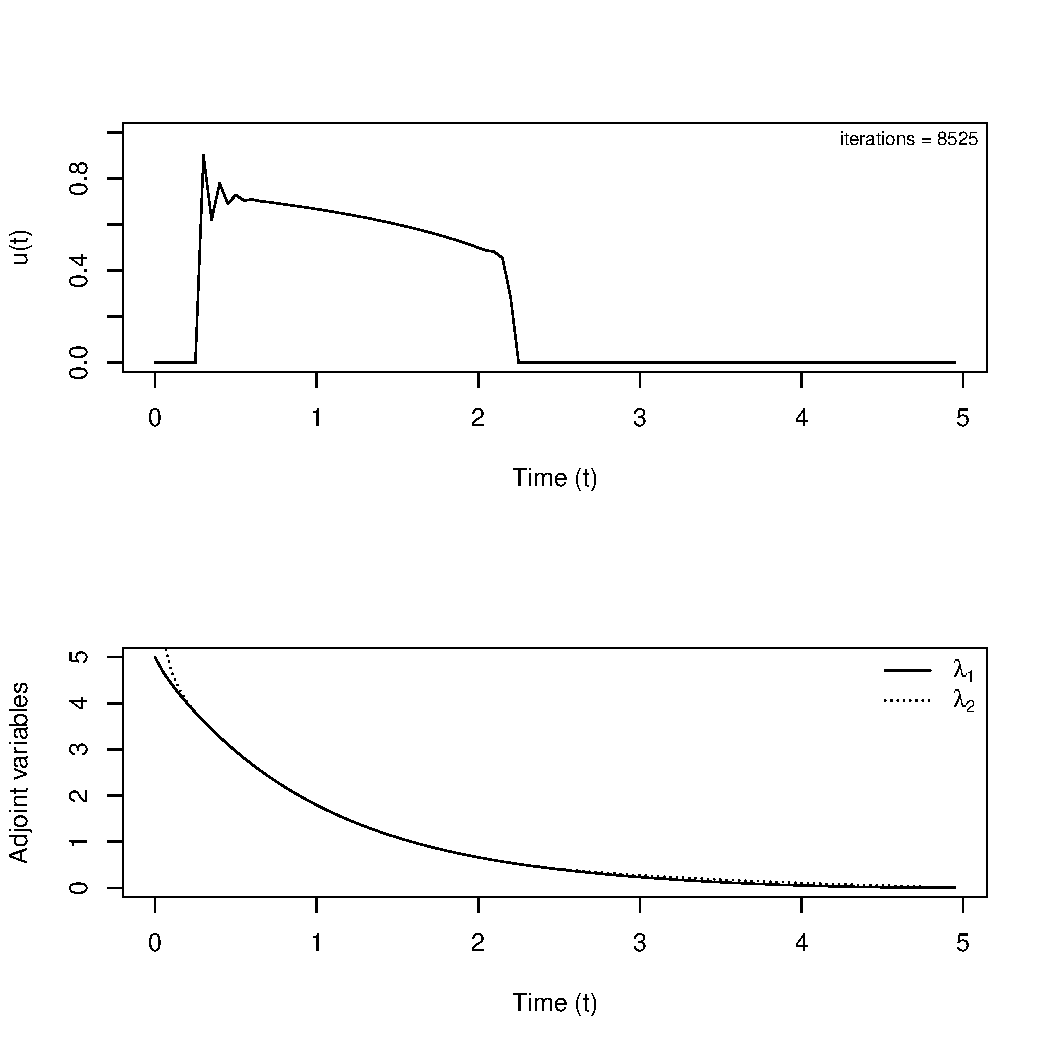
\includegraphics[page=1,width=.9\textwidth]{../../figures/forwardBackwardSweep-x1=1-x2=0}  
    \caption{ (A) The left panel shows the control $u(t)$ that maximizes $ \int_{0}^{T} log(x_2) dt. $ Here, $ T=5$ and $x_2(0)/x_1(0) = 0$. (B) The right panel shows the solution to the ODE for the control $u(t)$. [This figure corresponds to Figure 3 in King and Roughgarden (1982).] }
 \label{fig:kingRoughgardenFigure3}
\end{figure}

 \begin{figure}[h]
   \centering
       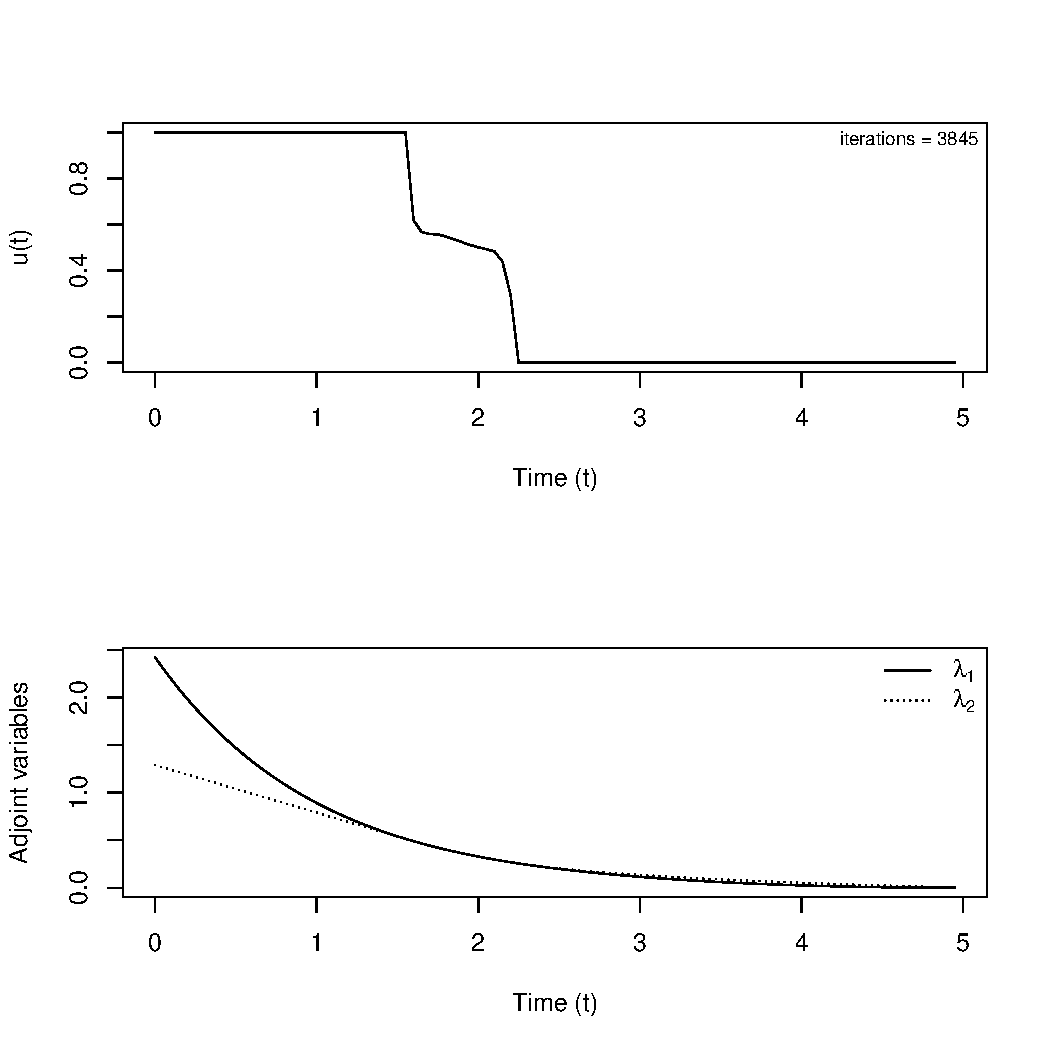
\includegraphics[page=1,width=.9\textwidth]{../../figures/forwardBackwardSweep-x1=1-x2=2}  
    \caption{ (A) The left panel shows the control $u(t)$ that maximizes $ \int_{0}^{T} log(x_2) dt. $ Here, $ T=5$ and $x_2(0)/x_1(0) = 2.0$. (B) The right panel shows the solution to the ODE for the control $u(t)$. [This figure corresponds to Figure 4 in King and Roughgarden (1982).] }
 \label{fig:kingRoughgardenFigure4}
\end{figure}

 \begin{figure}[h]
   \centering
       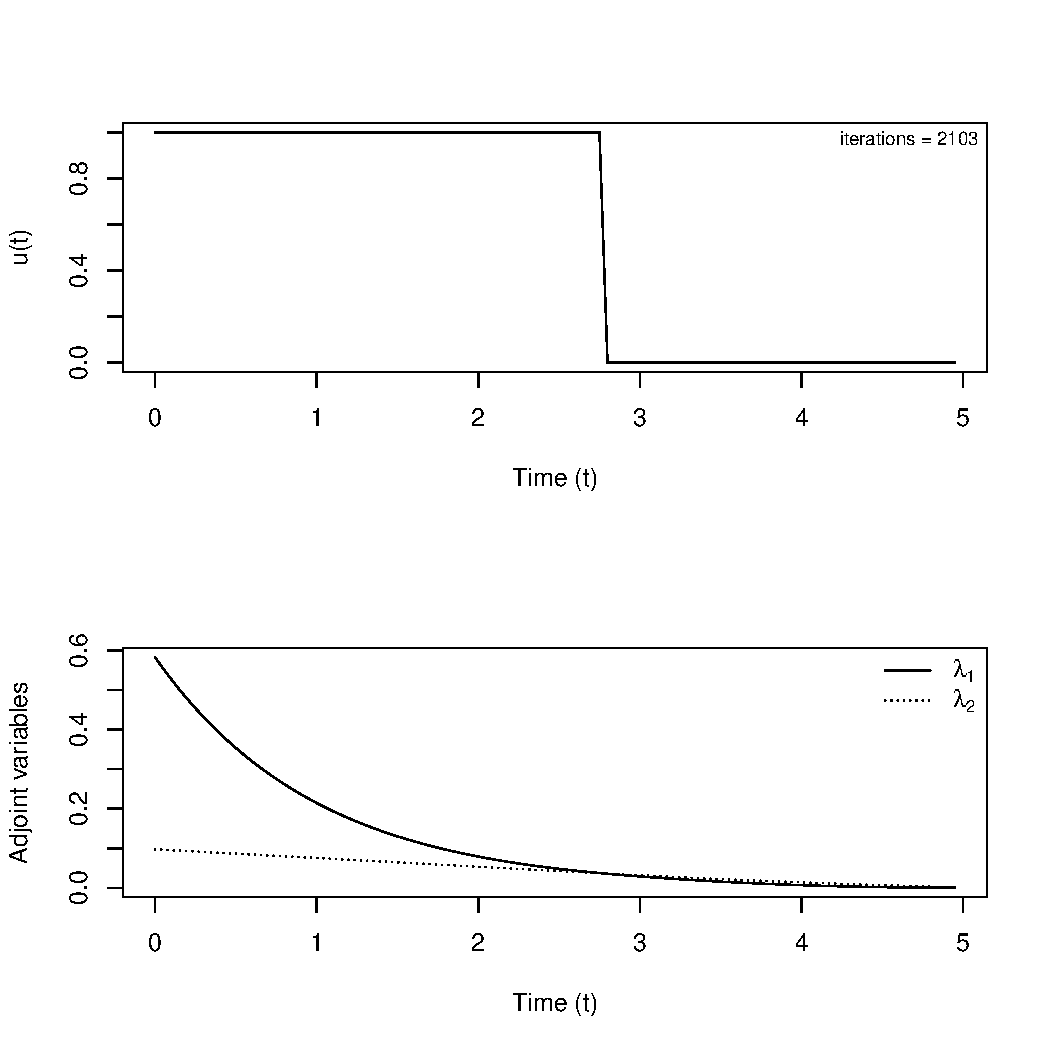
\includegraphics[page=1,width=.9\textwidth]{../../figures/forwardBackwardSweep-x1=1-x2=454}  
    \caption{ (A) The left panel shows the control $u(t)$ that maximizes $ \int_{0}^{T} log(x_2) dt. $ Here, $ T=5$ and $x_2(0)/x_1(0) = 45.4$. (B) The right panel shows the solution to the ODE for the control $u(t)$. [This figure corresponds to Figure 5 in King and Roughgarden (1982).] }
 \label{fig:kingRoughgardenFigure5}
\end{figure}


\clearpage
\section*{Changing the season length distribution}

To explore how changing the distribution of season length affects the optimal control, I modified the objective function. For a normal distribution of season lengths, the optimal control problem becomes:
\begin{align}
\max_{u} & \frac{1}{\Phi(T)-\Phi(0)} \int_0^T \frac{1}{\sigma \sqrt{2 \pi}} \exp{\big(-\frac{1}{2} (\frac{t-\mu}{\sigma})^2\big)} \log( x_2(t) ) dt \nonumber \\
\mathrm{subject\ to\ } & \dot{x_1} = u(t) x_1,\ \dot{x_2} = (1-u(t)) x_1, \nonumber \\ 
& x_1(0) > 0,\ x_2(0) \geq 0, \nonumber \\ 
& 0 \leq u(t) \leq 1.
\end{align}

This is equivalent to solving the problem with the following objective function:

\begin{align}
\max_{u} &  \int_0^T  \exp{\big(-\frac{1}{2} (\frac{t-\mu}{\sigma})^2\big)} \log( x_2(t) ) dt 
\end{align}

The Hamiltonian here is:
\begin{align}
H = \exp{\big(-\frac{1}{2} (\frac{t-\mu}{\sigma})^2\big)} \log( x_2(t) ) + x_1( \lambda_1 - \lambda_2 ) u(t) + x_1 \lambda_2
\end{align}

The season length distribution enters the problem in the objective function, which is independent of the control. For this problem, the optimality  
\begin{align}
\frac{\partial H}{\partial u} = x_1(\lambda_1 - \lambda_2) = 0\ \mathrm{at}\ u^* 
\end{align}

and transversality conditions
\begin{align}
\lambda_1(T) = \lambda_2(T) = 0
\end{align}

are the same as in the problem for uniformly distributed season lengths. The season length distribution changes the adjoint equations:
\begin{align}
&-\frac{\partial H}{\partial x_1} = \dot{\lambda_1}  = u(\lambda_2 - \lambda_1) - \lambda_2 \nonumber \\
&-\frac{\partial H}{\partial x_2} = \dot{\lambda_2}  = -\frac{  \exp{\big(-\frac{1}{2} (\frac{t-\mu}{\sigma})^2\big)}} {x_2}.
\end{align}

The script to find the optimal control using a forward-backward sweep algorithm is similar to that described for a uniform distribution of season lengths. However, I change the system of differential equations for the adjoint variables to correspond to the equations above and incorporate the distribution of season length. In solving the system of ODEs, time is used to calculate the control $u(t)$ and state variable $x_2(t)$. Time is also used to calculate the normal density at time $t$.

\begin{lstlisting}
###########################################################
# ODE for adjoint variables, lambda(t)
###########################################################
## The state x(t) must be an externally defined function [xFunc(t)]
backward = function(t,y,parms,f1,f2) {
  
  lambda1=y[1];
  lambda2=y[2];
  u = f1(t);
  x2 = f2(t);
  
  return(list(c((lambda2-lambda1)*u - lambda2, -(dnorm(t,mean=mu,sd=sigma)/x2) )))
}
\end{lstlisting}

 \begin{figure}[h]
   \centering
       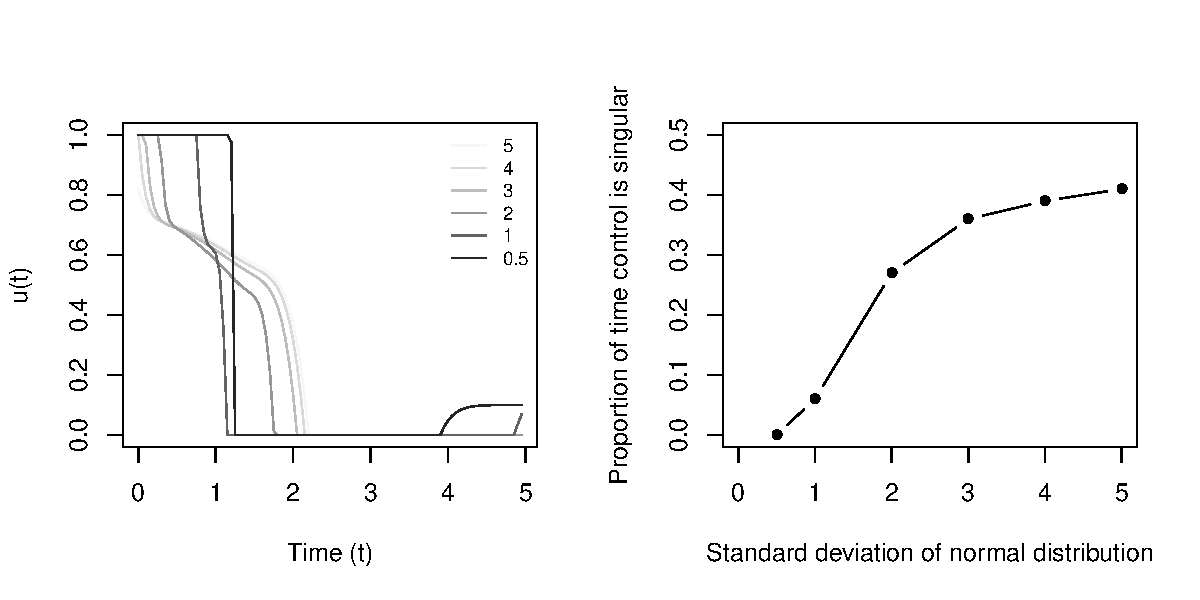
\includegraphics[page=1,width=.9\textwidth]{../../figures/kingRoughgardenNormalSummary}  
    \caption{ (A) The left panel shows the control $u(t)$ that maximizes $ \int_0^T  \exp{\big(-\frac{1}{2} (\frac{t-\mu}{\sigma})^2\big)} \log( x_2(t) ) dt. $ Here, $ T=5$ and $x_2(0)/x_1(0) = 0.25$ and each line corresponds to normally distributed season lengths with a mean of 2.5 and different values for the standard deviation, from 5 to 0.5. (B) The right panel summarizes the controls on the left by plotting the proportion of time the control is singular against the standard deviation of the season length distribution. This result is an example of the following conclusion from p. 12 of King and Roughgarden 1982: "We have also computed graded optimal controls for a Gaussian distribution of season length. As one expects, the shift to reproduction becomes more abrupt as the variance in season length decreases." }
 \label{fig:kingRoughgardenFigure4}
\end{figure}

\end{document}